\section{Results}
\label{sec:results}

\subsection{Synthetic mechanism check}
\label{sec:res-synth}
\begin{table}[t]
\centering\scriptsize\setlength{\tabcolsep}{2.5pt}
\resizebox{\columnwidth}{!}{\begin{tabular}{lcccc}\toprule
Case & Topology & $g(w)=w$ & Learned $g$ & corr$(g,\hat g)$ \\\midrule
linear & 0.50$\pm$0.00 & 0.92$\pm$0.05 & 0.93$\pm$0.03 & 0.996 \\
threshold & 0.50$\pm$0.00 & 0.91$\pm$0.01 & 0.95$\pm$0.04 & 0.982 \\
saturating & 0.50$\pm$0.00 & 0.87$\pm$0.03 & 0.88$\pm$0.05 & 0.969 \\
binary & 0.97$\pm$0.02 & 0.97$\pm$0.02 & 0.97$\pm$0.02 & -- \\
regions (node-only AUROC) & \multicolumn{3}{c}{0.80$\pm$0.05} & top-4 prec. 0.95 \\
\bottomrule\end{tabular}
}
\caption{Synthetic test AUROC (mean$\pm$SD, five seeds). corr$(g,\hat g)$ is Pearson correlation
over the 5th--95th percentile of observed training weights; last row: node-only W-GNAN AUROC and top-4 precision for planted regions.}
\label{tab:synthetic}
\end{table}

Each seed generated 700 balanced 36-node graphs (420/140/140 train/validation/test), Beta$(2,2)$
weights, noise SD $0.12$ times latent-score SD, and one topology shared across splits (except the
binary case, which varies topology). Graph cases set $u_i$ to a learned centred region constant to
isolate the interaction channel. The topology-only model is at chance for the three fixed-topology
cases, while weighted variants reach 0.87--0.95 (Table~\ref{tab:synthetic}). Learned $g$ tracks the
generating shape over observed support (Figure~\ref{fig:synthetic}; correlations .969--.996). Its threshold-case advantage over
fixed $g(w)=w$ is descriptive ($.95\pm.04$ vs. $.91\pm.01$), not a formal superiority test. With
binary weights, all variants coincide within numerical precision, and node-only W-GNAN retrieves the
four planted regions with top-4 precision .95.

\begin{figure*}[t]
\centering
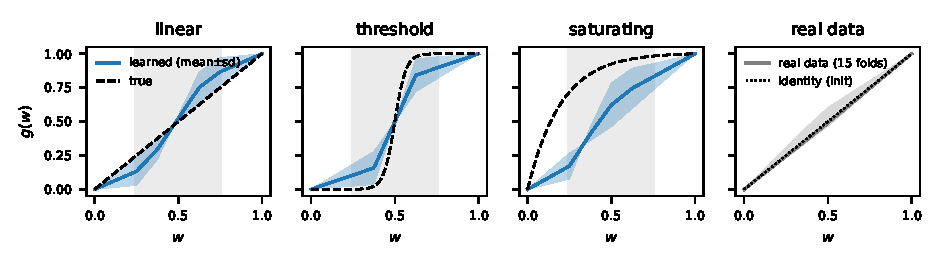
\includegraphics[width=.86\textwidth]{figures/fig2_synthetic_v2b.pdf}
\caption{Learned $g$ (mean$\pm$SD across five seeds) against the generator; grey shading marks the
observed-weight support on which correlation is reported. Right: real-data fold curves remain near
their identity initialization, a training diagnostic rather than evidence that no nonlinear signal
exists.}
\label{fig:synthetic}
\end{figure*}

\subsection{Probable-PTSD benchmark}
\label{sec:res-bench}
\begin{table}[t]
\centering\scriptsize\setlength{\tabcolsep}{2.5pt}
\resizebox{\columnwidth}{!}{\begin{tabular}{lccc}
\toprule
Model & AUROC & AUPRC & $\Delta$AUROC \\
\midrule
Majority & 0.500 [0.50, 0.50] & 0.069 [0.05, 0.09] & $-0.087$ [$-0.15$, $-0.02$] \\
LR edges & 0.588 [0.52, 0.65] & 0.093 [0.07, 0.14] & -- \\
LR strengths & 0.572 [0.50, 0.64] & 0.099 [0.07, 0.15] & $-0.017$ [$-0.06$, $+0.03$] \\
GAT$^\ast$ & 0.539 [0.46, 0.62] & 0.089 [0.06, 0.15] & $-0.030$ [$-0.12$, $+0.07$] \\
GCN$^\ast$ & 0.515 [0.44, 0.60] & 0.075 [0.05, 0.11] & $-0.054$ [$-0.12$, $+0.01$] \\
W-GNAN node-only & 0.558 [0.51, 0.61] & 0.083 [0.06, 0.11] & $-0.029$ [$-0.09$, $+0.03$] \\
W-GNAN binary topo. & 0.552 [0.49, 0.61] & 0.088 [0.07, 0.12] & $-0.037$ [$-0.10$, $+0.03$] \\
W-GNAN $g(w)=w$ & 0.565 [0.50, 0.63] & 0.094 [0.07, 0.13] & $-0.024$ [$-0.08$, $+0.04$] \\
W-GNAN learned $g$ & 0.584 [0.52, 0.65] & 0.097 [0.07, 0.14] & $-0.005$ [$-0.07$, $+0.07$] \\
\bottomrule
\end{tabular}
}
\caption{Held-out performance (60/869 positives). AUROC/AUPRC are repeat means; intervals are
1,000-resample subject-cluster bootstraps. Deltas are paired with LR edges; GNN deltas pair repeat 0
only. AUPRC prevalence is .069. $^\ast$Repeat 0 only, on low-CV sparsified inputs (\S\ref{sec:setup}).}
\label{tab:benchmark}
\end{table}

LR edges exceeds the constant-score majority reference in the paired comparison
($\Delta=.087$ [.02, .15]) and reaches AUROC .588 [.52, .65] (Table~\ref{tab:benchmark}). W-GNAN
learned $g$ reaches .584 [.52, .65], with paired $\Delta=-.005$ [$-.07,.07$]; this interval neither
resolves a difference nor establishes equivalence. The fixed-weight and topology ablations are lower
but their paired intervals include zero, so they do not establish that weighting is irrelevant. GAT
(.539) and GCN (.515) reflect only the stated sparsification and one-repeat design.

\subsection{Diagnostics and selected nuisances}
\label{sec:res-sanity}
\begin{table}[t]
\centering\scriptsize\setlength{\tabcolsep}{2.5pt}
\resizebox{\columnwidth}{!}{\begin{tabular}{lcc}
\toprule
\multicolumn{3}{l}{\emph{Classification (PCL-5 $\geq$ 33)}} \\
Model & AUROC [95\% CI] & $\Delta$AUROC vs.\ LR edges \\
\midrule
LR: scale only (total, density) & 0.487 [0.42, 0.55] & $-0.101$ [$-0.183$, $-0.004$] \\
LR: age + sex & 0.452 [0.40, 0.50] & $-0.135$ [$-0.21$, $-0.06$] \\
LR edges, old log1p pipeline & 0.595 [0.52, 0.66] & $+0.006$ [$-0.03$, $+0.04$] \\
LR edges, age/sex/total removed & 0.583 [0.52, 0.65] & $-0.005$ [$-0.02$, $+0.01$] \\
\midrule
\multicolumn{3}{l}{\emph{Regression on PCL-5 score}$^\dagger$} \\
Model & MAE & $R^2$ / Spearman $\rho$ \\
\midrule
Constant (predict 3) & 8.09 & -- \\
Ridge on edges & 9.40 & $-0.000$ / 0.031 ($p=0.35$) \\
\bottomrule
\end{tabular}
}
\caption{Selected checks. Classification uses the final repeated-CV protocol. $^\dagger$Regression
is from an earlier five-fold pipeline and is not directly comparable with Table~\ref{tab:benchmark}.}
\label{tab:sanity}
\end{table}

Age/sex and total-streamline/density models have AUROC .452 and .487; train-fold residualisation on
age, sex and total streamlines changes LR-edge AUROC by $-.005$ [$-.02,.01$]. These checks find no
predictive contribution from those measured variables under the tested linear controls; they do not
rule out all confounding or nonlinear interactions. Exploratory cutoffs 30/25/20 yield strength-LR
AUROC .53--.56 (separate five-fold CV; all intervals include .5). Earlier continuous-score ridge
regression is worse than a constant in MAE (9.40 vs. 8.09). Across the 15 W-GNAN folds, $\lambda$
stays near its initial 1 (median .97) and $g$ near identity (Figure~\ref{fig:synthetic}, right). This is an optimization diagnostic, not proof that the cohort lacks weight-dependent
signal.

\subsection{Region-level interpretability audit}
\label{sec:res-interp}
\begin{figure*}[t]
\centering
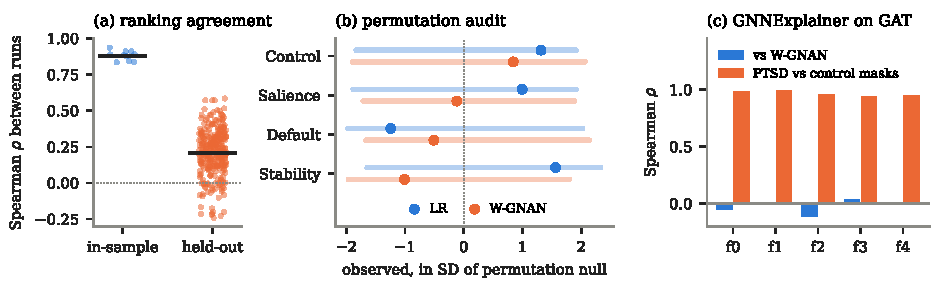
\includegraphics[width=.86\textwidth]{figures/fig4_interp.pdf}
\caption{Region-level audit. (a) Mean pairwise Spearman correlation between rankings from five
all-subject seeds of an earlier prototype and from its 25 held-out fits. (b) Observed statistics standardized by their own permutation-null mean
and SD; bars show null 95\% intervals. (c) Per-fold Spearman $\rho$ of positive-subject GNNExplainer node masks with $|t_i|$ group
differences (blue) and with control-subject masks (orange).}
\label{fig:interp}
\end{figure*}

The earlier prototype's all-subject seed rankings agree strongly ($\rho=.88$), whereas rankings from
its held-out fits agree weakly ($\rho=.21$; Figure~\ref{fig:interp}a). Because architecture, training population and sample size
also differ, this contrast demonstrates non-replication in that pipeline but does not isolate subject
reuse as the cause. For the final audit (Figure~\ref{fig:interp}b), stability does not exceed its label-permutation null (LR
$p=.07$; W-GNAN $p=.85$), and no hypothesis-motivated network crosses $\alpha=.0167$
(Control/Salience/Default: LR $p=.10/.16/.88$; W-GNAN $p=.22/.56/.67$). Resolution is .002 for LR
and .010 for W-GNAN; non-significance is not equivalence or evidence of no biological effect.

GNNExplainer's nonnegative node masks are compared per fold with absolute W-GNAN region allocations (Figure~\ref{fig:interp}c):
mean Spearman $\rho=-.03$ (range $-.12$ to $.04$) and top-30 overlap 1.4 regions (chance 2.1, continuous
masks ranked by deterministic order). Positive/control masks are nearly identical ($\rho=.96$) and
positive-mask stability across folds is .94; the explained-set GAT AUROC is .48. Mask
stability therefore does not establish label-specific information, and mask sign/direction is
not recoverable.
